\section{QR Search Results}

\begin{frame}{On QR Data, Bird-BM Uses the Fewest Comparisons}
\centering
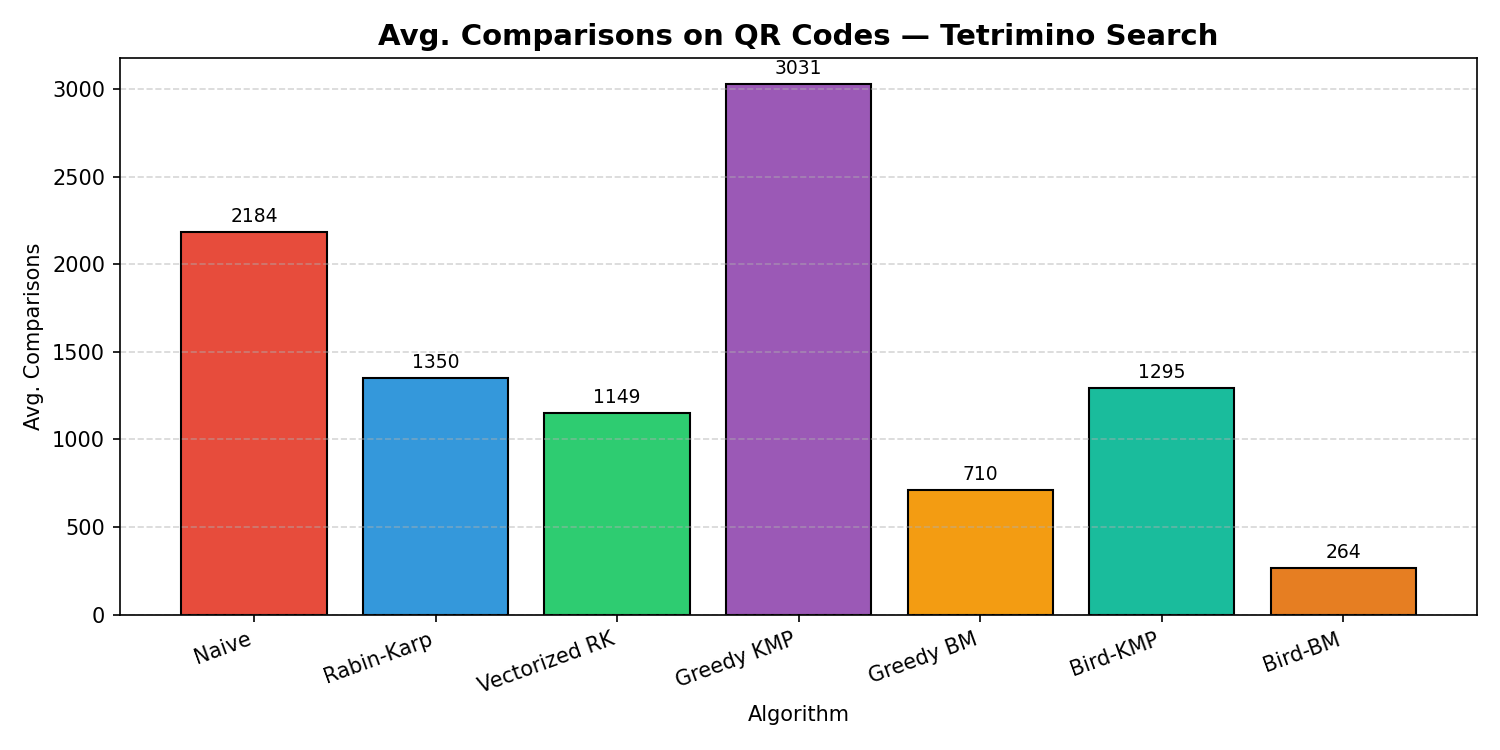
\includegraphics[width=\linewidth,height=0.50\textheight,keepaspectratio]{qr_avg_comparisons.png}

\vspace{0.3em}
\keymsg{Best average comparison count: \textbf{\QrBestCompAlgo{}} (\QrBestCompValue{}).}
\sourcenote{\texttt{results\_qr.csv} and \texttt{qr\_avg\_comparisons.png}}
\end{frame}

\begin{frame}{Greedy BM Dominates Runtime on QR Inputs}
\centering
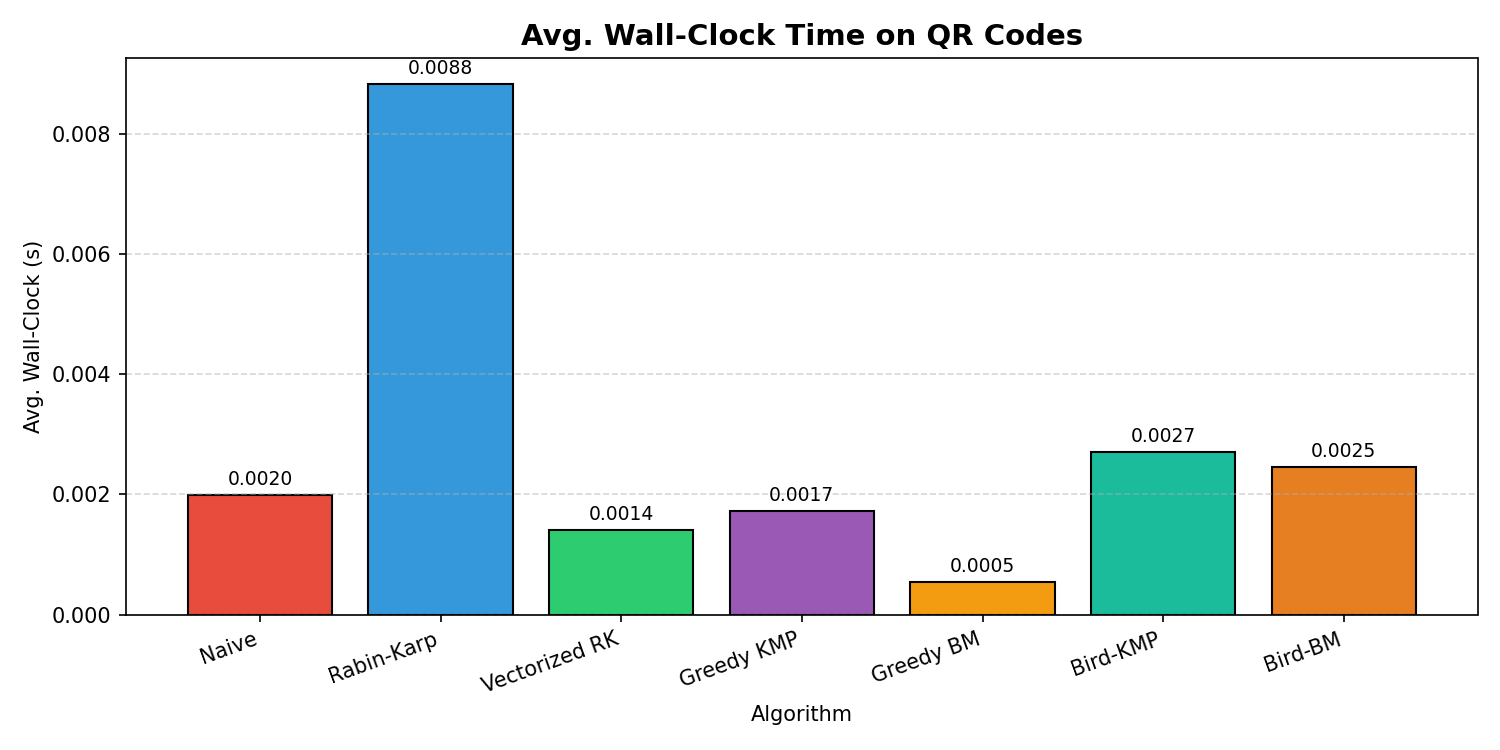
\includegraphics[width=\linewidth,height=0.50\textheight,keepaspectratio]{qr_wallclock.png}

\vspace{0.3em}
\keymsg{Fastest average runtime: \textbf{\QrBestTimeAlgo{}} (\QrBestTimeValue{} s).}
\caveat{Bird-BM wins comparisons but is slower due to implementation overhead.}
\sourcenote{\texttt{results\_qr.csv} and \texttt{qr\_wallclock.png}}
\end{frame}

\begin{frame}{Per-Image Stability Across \QrImageCount{} QR Inputs}
\centering

\includegraphics[width=\linewidth,height=0.46\textheight,keepaspectratio]{qr_per_image_comparisons_focus.png}

\vspace{0.3em}
\begin{block}{Observation}
The ordering is consistent across images: Bird-BM remains lowest in comparisons, while Greedy BM stays competitive with lower runtime.
\end{block}
\sourcenote{\texttt{results\_qr.csv} and \texttt{qr\_per\_image\_comparisons.png}}
\end{frame}

\begin{frame}{QR Section: Corrected Numeric Callouts}
\small
\begin{itemize}
  \item Mean comparisons (Rabin-Karp): \textbf{\QrCompRabinKarp{}}.
  \item Mean comparisons (Vectorized RK): \textbf{\QrCompVectorizedRK{}}.
  \item Mean runtime (Greedy BM): \textbf{\QrTimeGreedyBM{}} s.
  \item Mean runtime (Vectorized RK): \textbf{\QrTimeVectorizedRK{}} s.
\end{itemize}

\begin{block}{Data integrity note}
These values are recomputed directly from \texttt{results\_qr.csv}, superseding stale summary values.
\end{block}
\caveat{Raw \texttt{qr/} images are not in this repo snapshot; evidence is chart/CSV based.}
\end{frame}
